% !TeX spellcheck = en_GB

\section{Features and methods for \acrshort{asc} and \acrshort{aedc}}
\label{section:features-and-methods-for-asc-aedc}
	
	As in many fields, the boundaries between features and methods used for audio tasks are becoming blurred since the recent rise of deep learning based methods. Classically, a problem is addressed with a pre-processing stage of the data and then the model or method is implemented. Right now, these two stages are sometimes maintained but also have been mixed or changed depending on how the algorithm works.

%\subsection{Features}
%\label{subsection:features}

	In every machine learning or pattern recognition task, for the system to be able to infer and extract conclusions from the input given, a pre-processing stage is necessary to make some transformations to the data so that they could be understood by the model. This stage is known as feature extraction and the goal is to convert the original information into a set of values or vectors that characterize the data regarding some desired properties \cite{Giannakopoulos2014}.
	
	There are several ways that allow us to perform this processing stage. The most common and basic one consists on extracting features that are closely related to the original signal which are called \acrfull{lld}  \cite{Amatriain2004}. These are computed by performing some mathematical operations or formulas to the original data and can be considered rudimentary when comparing with other techniques. However, they are really extended and still in use nowadays \cite{Marr1982}. 

	In the audio field, there are two types in which all \acrshort{lld} can be grouped into. One of them is for the features that have been computed by considering the audio signal in its original form in the recording, i.e., in time-domain, that is the reason why they are known as time-domain audio features. The other case refers to those characteristics that are obtained from the signal after having been transformed into the frequency domain. These are commonly known as frequency-domain or spectral audio features. For the procedure of feature extraction, the signal is usually divided into frames that can be overlapped by using a sliding window, so the calculations are done per frame, obtaining a final matrix with size $number\ of\ frames \times number\ of\ features$ \cite{Giannakopoulos2014}. It must be taken into account that the goal of the whole system is going to be fundamental at the time of deciding which features must be computed. For example, not the same features are to be used for speech recognition than for musical information retrieval. In table \ref{table:6}, a summary of most used time and spectral features is included.
	
	% Table of time domain features
	\begin{table}[h!]
		\begin{center}
			\centering
			\begin{tabular}{|| m{9em} | m{24em} ||}
				\hline
				\begin{center}\textbf{Feature}\end{center}& \begin{center}\textbf{Description}\end{center} \\
				\hline\hline
				\multicolumn{2}{||c||}{\textbf{Time}} \\
				\hline
				Energy Entropy & It is useful to detect sudden changes from the energy of a signal. To calculate this value for a certain subframe, it is necessary to first compute the normalized energy of the subframe with respect to all the frames energy \cite{Giannakopoulos2006}. \\
				\hline
				Short time energy & It is the energy for a short segment of signal. It is normally used in speech-related tasks in order to identify voiced form non-voiced fragments \cite{Garcia-Gomez2016}, among other things. \\
				\hline
				\acrfull{zcr} & This can be defined as the number of times the amplitude of the signal crosses the zero line per unit of time, i.e., changes from negative to positive. It is sometimes computed by the number of zero-crossings by the amount of samples in the frame \cite{Giannakopoulos2006}. \\
				\hline
				\multicolumn{2}{||c||}{\textbf{Frequency}} \\
				\hline
				\acrfull{sf} & It is computed to measure the spectral changes between two successive frames. To do so, the difference of their spectral energy obtained from the \acrshort{fft} is computed \cite{Garcia-Gomez2016}.  \\
				\hline
				Spectral Rolloff & This represents the skewness of the shape of the spectrum given the frequency below which a concrete percentage of the magnitude distribution of the frequency transform is concentrated \cite{Garcia-Gomez2016}. \\
				\hline
				\acrfull{sc} & This is a measure related to the spectral position. It is defined as the center of gravity of the spectrum. %, i.e., \doubt{it indicates how high the spectrum values are on average} 
				\cite{Giannakopoulos2006}. \\
				\hline
				\acrshort{mfcc} & It is a feature that it is widely used because it gives good results in many tasks as for example, speech recognition since it interprets the frequency bands in a very similar way to human perception while doing a separation of the fine structure of the spectra (that corresponding with the harmonics) and the coarse (i.e. the filter representing the vocal tract). It is computed from the \acrshort{stft} \cite{Garcia-Gomez2016}. A wider explanation can be found in appendix \ref{appendix:spectrogram-mel-scale}. \\
				\hline
			\end{tabular}
		\end{center}
		\caption{Examples of time  and spectral audio features.}
		\label{table:6}
	\end{table}

	Moreover, either time-domain or spectral features can also be split in two groups depending on the way the were extracted. There are the ones called short-term features. This way of computing follows the framing process explained above. The signal is initially divided in various frames that are commonly overlapped and for each frame the feature is calculated \cite{Giannakopoulos2014}. The other case refers to long-term features. This way the different computations to obtain the descriptors are performed along longer segments, sometimes the whole audio is took \cite{BUYUK2018}. For a certain long sequence, the computation of the short term features are calculated and then some statistics are performed in order to characterize this information for the long term. Actually, the long-term sequence can be defined as a set of statistics that resumes the short-term features for a sequence. The portion of audio selected for the long-term usually presents a uniform behaviour within the total data \cite{Giannakopoulos2014}.

	To sum up, a typical procedure would first divide the signal into frames. The next step would be to compute the short-term features considering some time-domain or spectral characteristics within the audio data that are thought to be determinant in the required task. Finally, a series of mathematical and statistical transformations are performed in order to obtain a \acrshort{lld} vector per sample in order to pass these input data to a statistical model that will be trained with the objective of summarizing the properties of the signals and develop a classification rule so as to be able to assign a faithful category to a new unlabelled observation \cite{Stowell2015}. For example, some of the long-term features that can be obtained from the short-term ones included in \ref{table:6} could be the variance and mean in the case of short time energy, or the relation between the maximum and the mean along the frame for the \acrshort{sf} \cite{Giannakopoulos2006}.
		
	A common approach for the utilization of this type of \acrshort{lld} in the long-term way is the one known as \acrfull{bof}. The term has been acquired from the text treatment field as an analogy to the technique known as "bag-of-words", which consists on treating the text data as a global and unique distribution of words without giving importance to their order inside the sentences \cite{Uijlings2009}. The analogous system for audio tasks consists in representing signals as statistics of long-term sequences of their spectral local features. This method has been applied in different fields in the \acrshort{asc}, for example, in order to analyze "soundscapes", analogy for audio landscape, and polyphonic music \cite{Aucouturier2007}. It was established that this approach was a proper option in order to work with soundscapes since the order of the audio sequence inside of them was not really relevant for its understanding. However, in the music task, the ordering of the parts of the sound was determinant to retrieve the musical information, so the technique was discarded for this topic \cite{Aucouturier2009}. A common way of exploiting this concept of \acrshort{bof} is by using the already mentioned \acrshort{mfcc} and the really well-known technique in the literature as \acrshort{gmm}. These are generative methods in which the feature vectors are treated as they were produced by a multimodal distribution which consists on a sum of Gaussian distributions \cite{Barchiesi2015} \todo{check}. In figure \ref{fig:mesh53}, it is shown the structure of a \acrlong{bof} approach. 
	
	\begin{figure}[H]
		\centering
		\captionsetup{justification=centering}
		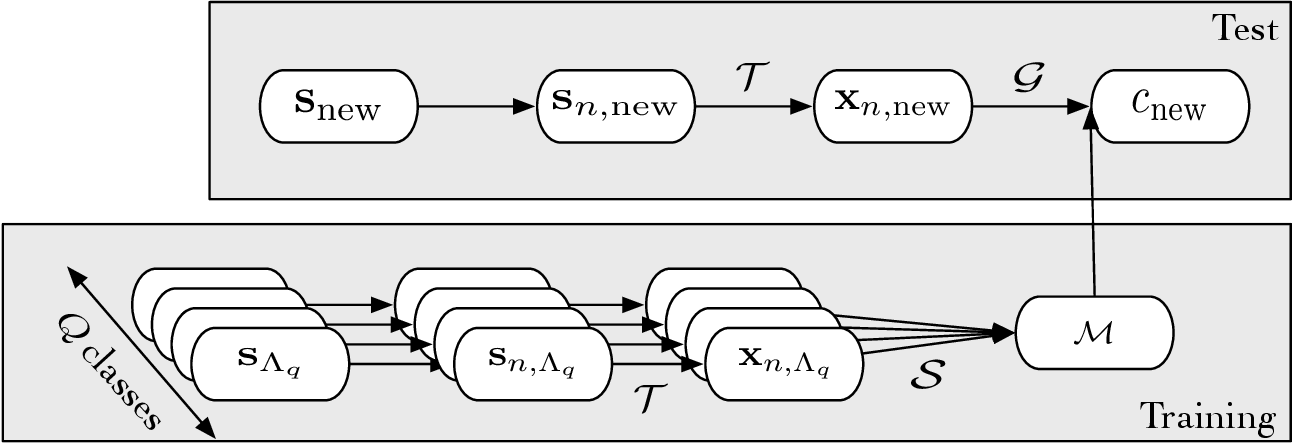
\includegraphics[scale=0.32]{bof-gmm}
		\caption{Framework for ASC addressing the idea of BOF and using a GMM to obtain statistical representation of the low-level features. $S_{\Lambda q} $ are the original labelled samples in the training set and $S_{n,\Lambda q}$ multimodal distributions for these samples. $x_{n,\Lambda q}$ are the features extracted with an operator $T$ which are taken by an operator $S$ to learn the global model $M$. Then, in the testing process, a likelihood measure $G$ is used in order to classify the \textit{new} sample.}
		\label{fig:mesh53}
	\end{figure}
	
	A similar way of acting can be found for \acrshort{aed}. In this case, the typical procedure has been found to be defined as a two-steps process. For the case of \acrfull{med} \cite{Wang2016}, in the first part, some features are generated at a clip level, usually by concatenating frame-level features, so then, in the second stage, a binary or multiclass classification can be done in order to confirm the presence of an event in a whole clip of video. This idea follows the same concept of \acrshort{bof} explained above since the generation of features do not attend to their order in the whole clip.
	
	Another similar approach has been found for this task, but in this case it differs from the \acrshort{bof} and it is applied to real-life recordings. For the first stage, a classification of already isolated events is performed so a vocabulary of acoustic actions can be built. For this purpose, it is needed a set of short-term video recordings in which the semantic meaning of the corresponding audio event must be clear and highlighted over all the others sounds that take place along the sequence. In the second stage, the detection procedure takes place along the whole clip by making use of the previous configured vocabulary of acoustic data \cite{Mesaros2010}. The way the events are modeled in this task is by using \acrfull{hmm}. This is a common technique that has been put in practice plenty of times in the audio world and consists in modeling the temporal succession of the events within a longer sequence. This can be done by saving the order of the events in a transition matrix that contains the probability of one sound occurring after another one \cite{Barchiesi2015}.
	
	Also, this process can be combined with a classification of the events detected during the long sequence in order to make an \acrshort{asc} based on what type of sounds are taken place within the scene \cite{Barchiesi2015}. This is actually the initial idea desired for our work. Building a violent acoustic dictionary with a classification of monolabel short time recordings so as to then perform a detection process for violent acoustic events in order to categorize the scene and check if there is violence on it. However, we just mainly made an approach for the very first part about classifying what we considered violent events. This will be explained further on in \ref{chapter:our-approach-for-avd} and \ref{chapter:experiments}.
	
	In some cases, the mentioned \acrlong{lld}, sometimes referred as manually-crafted features, are not enough to model data since they cannot achieve a meaningful representation of the original information for the system to learn from. Also, as mentioned above, the selection process of this type of features plays a significant role in the final output so that the criteria of the designer could be considered a limitation for the classification task \cite{Grill2012}. For this reason, a new strategy of addressing feature extraction has appeared based on the idea of finding more specialized properties by using specific engineering algorithms that explores the given data in order to find non-human recognizable patterns. The techniques that allow to perform this task are usually called automated feature generation algorithms or machine-learnt features \cite{Pachet2009}.
	
	In order to compute these high-level features, there is not just one standardized machine model that allow to compute them all in a particular form. The calculation method, nevertheless, differs from one approach to another. One example could be the combination of low-level data with high-level semantic descriptors that consists on the inference of diverse dimensions by using \acrlong{svm}s so as to find similarities among music genres. Particularly, they consider the output probabilities of the \acrshort{svm} classifier as a high-level feature space in which the distance between samples from different classes can be measured \cite{Bogdanov2011}. This algorithm has been one of the most popular ways to track classification problems.
	 
	There are plenty of works in the literature that use this technique for audio classification tasks \cite{Jiang2005} \cite{Geiger2013} \cite{Barchiesi2015}. It is originally known to be a binary classifier but, nowadays, there have been some implementations that allow its use it in multiclass problems. This algorithm makes the classification by taking into account pairs of observations that are more likely to be misclassified and draws a hyperplane as the optimal boundary between the two classes \cite{Fu2011}. Since it has been used for the experiments in this work, a more detailed explanation will be included in section \ref{section:models}.
	
	Several methods that have been really successful on the high-level feature extraction apart from other tasks as detection and classification lay under the umbrella of \acrfull{ann}. This concept was inspired by human biology and how the neurons communicate among them in the brain in order to interpret the input or sensory data humans collect. 
	
	In the field of \acrshort{aed} these have been used in order to implement techniques also for automatic learning of features. For example, a technique of boosting is used to extract discriminative features which resulted in a better performance than \acrshort{mfcc} for real-life acoustic data \cite{Zhuang2010}. They first made an attempt based on modeling the sequence data with \acrshort{hmm} explained before and combined them with a trained \acrshort{ann}. Also, an approach based on \acrshort{svm} and \acrshort{gmm} was tried. 
	
	The development of the \acrshort{ann} in different ways has made possible the implementation and creation of new algorithms during the last years that exploits the concept of neural models from different perspectives. Is the case of \acrfull{cnn}, which follows the way of working of the neural networks but performing convolution operations over the input data \cite{Fu2011}. This has achieved really good results for image tasks in the \acrlong{cv} field, but also implemented successfully in audio problems. As in \cite{Ren2018}, where is proposed a method based on \acrshort{cnn} in order to classify ten acoustic scenes. In order to feed the model they used log-mel spectrogram images. More information about this type of data can be found in appendix \ref{appendix:spectrogram-mel-scale}. A detailed explanation of \acrshort{cnn} can be found in subsection \ref{subsection:ann-cnn}.
	
	Also, another type of networks that has been treated largely with the purpose of working with sequential data is the \acrfull{rnn}. The concept behind these models is its capability of being able to learn information from previous elements inside a sequence. Also, an adaptive model was designed called \acrshort{lstm}, which do basically the same but for longer sequences. One possible approach for this algorithms could be the one presented in \cite{Wang2016}. They first classify frame level audio against a set of semantic units. Then, the output is taken as a representation with variable length in a clip level which feed the \acrshort{lstm} as input. The results overtake \acrshort{svm} and \acrshort{fc} in similar tasks. More information about this type of networks is included in detail in subsection \ref{subsection:rnn-lstm}.
	
	Related to the development of these more complex models as \acrshort{cnn} or \acrshort{lstm}, a novel type of feature has been used in the last years that differs from the already explained low-level and high-level ones: \acrfull{dnn} have grown increasingly for plenty of classification tasks and so in the multimedia area. The problem with this type of systems is the huge amount of data that is needed to make them work properly, which can be translated in a lack of labelled data. One of the habits that has been currently resorted by the researchers consists of learning what is called deep data \textit{embeddings} from extensive collections of, in our case, audio and use them so as to perform shallow classifications by using simpler datasets. There have been implemented some models about this topic, such as \acrfull{l3} \cite{Cramer2019} net that uses as input for the the embedding extractor the linear-frequency log-magnitude spectrogram of 60 million audio samples, the system called SoundNet \cite{Aytar2016} that has been designed to obtain embeddings from training a deep audio classifier in order to predict the output o a deep image classifier and the \acrshort{vgg}ish network, designed by Google researchers. This last case is the one we used in this work and it will be explained in more detail in section \ref{section:feature-extractor}.
	
%	\todo{CPM: aquí hace falta que pongas ejemplos de feature extraction en AED. Basta un párrafo con dos o tres refs. Si no, no se sabe qué relación tiene esto con nuestro problema y cual es el estado del arte en nuestro problema en particular. Creo que todo esto lo tienes en el Features and Methods antiguo que ahora voy a leer. Creo que deberías cambiar el título de la sección 2.1.1 por 2.2 Features and methods for ASC and AED/C y complementarlo con las de la sección 2.1.2}
	
%\subsection{Classification models}
%\label{subsection:classification-models}

%\todo{remove this limitation, not the content just the subsection title to make all a subsection}
	
%Several algorithms have been designed in order to perform a classification task by finding patterns from input data features. Next we will present briefly some of the most commonly used in the literature and then provide a more detailed description of those we have used in this project. In particular, the most basic methods to tackle the classification task are \acrshort{knn}, \acrshort{svm} and also \acrshort{gmm} \cite{Fu2011}.
	
%	In the case of \acrfull{knn}, given a set of samples ${x_1, ..., x_n}$ that belong to a metric space $X$ whose labels are ${\theta_1, ..., \theta_n}$ respectively, if a new sample $x$ comes in, it will be categorized by following a majority vote process of the nearest neighbours considering a distance in the space $X$. A trade-off must exist in the choice of the number of nearest neighbours since on the one hand, it is desirable for it to be large so that the voting process has more participants and  the probability of misclassification is minimized and on the other, a small value with respect to the total number of samples so the nearest points are close enough to the new observation \cite{Cover1967}. \todo{Complete with example in the ASC or AEDC approaches. CPM: ok. Do not forget about it.}
	
%	 \acrfull{gmm} are a class of soft clustering methods. They are commonly used to derive global statistical properties from the feature vectors of the sample data. Specifically, considering $K$ clusters, they define a group of feature vectors from training data belonging to a certain category $q$ and model them as a multivariate normal distribution $N(\mu_k, \Sigma_k)$ that is further weighted by the probability $w_k$ of a particular certain observation to belong to cluster $k$. After learning a global model for the training data $M_q={w_k, \mu_k, \Sigma_k}$, a new observation will be categorized by applying the maximum likelihood criterion \cite{Stowell2015}. This technique is commonly used to extract statistical representation of local feature vectors to work with the audio data by following the idea of the \acrshort{bof} approach explained above in subsection \ref{subsection:features}.
	 %\todo{CPM: ok pero, ¿sabes qué estás diciendo si te preguntan?}
	
%	However, the one that has been generally more successful is the \acrfull{svm} classifier \todo{CPM: pero esto será cierto en un determinado campo, ¿no? Yo no sería tan rotunda diciendo esto salvo que pongas una cita apoyándolo o lo delimites a un campo en particular.}. There are plenty of works in the literature that use this technique for audio classification tasks \cite{Jiang2005} \cite{Geiger2013} \cite{Barchiesi2015}. It is originally known to be a binary classifier but, nowadays, there have been some implementations that allow its use it in multiclass problems. This algorithm makes the classification by taking into account pairs of observations that are more likely to be misclassified and draws a hyperplane as the optimal boundary between the two classes \cite{Fu2011}. Since this technique has been used for the experiments in this work, a more detailed explanation will be included in section \ref{section:models}.
	
%
%	
%	\todo{Mention applications of lstm and cnn. Also the paper in which both of them are combined}
%
%	\todo{Include image of FCC? CPM: ¿FCC? Do you mean FC or a DNN? It could be a good idea }
	

%Some other applications example could be building high-level feature detectors for image recognition by using unlabelled data to feed a \acrfull{nn} model \cite{Le2013}.
	
	
	
	

	
	
	
	
	
	
	
	